\documentclass{beamer}

\mode<presentation> {
\usetheme{Madrid}
\usecolortheme{beaver}
\setbeamertemplate{footline}[page number] % To replace the footer line in all slides with a simple slide count uncomment this line
\setbeamertemplate{navigation symbols}{} % To remove the navigation symbols from the bottom of all slides uncomment this line
}

\usepackage{graphicx}
\title[Sensors Assignment 3]
{Scortec ER-I Manipulator Control using Arduino Due}
\author
{Chittaranjan Srinivas Swaminathan \& Anders Wikstrom}
\institute{Orebro University}
\begin{document}
\frame{\titlepage}
  \begin{frame}
    \frametitle{Outline}
    \begin{enumerate}
      \item Description of the task
      \item Required steps
      \item Reverse Engineering
        \begin{itemize}
          \item Pinout diagram
          \item Encoders and debouncing
        \end{itemize}
      \item Control
        \begin{itemize}
          \item Velocity Control
          \item Position Control
          \item Calibration
        \end{itemize}
      \item Accuracy and precision
        \begin{itemize}
          \item Measurement 
          \item Control
        \end{itemize}
    \end{enumerate}

  \end{frame}
  \begin{frame}
    \frametitle{The task}
    \centering
    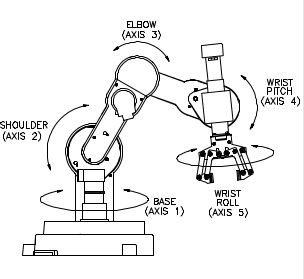
\includegraphics[scale=0.75]{../Report/axes.png}
    \begin{itemize}
      \item<1-> Scortex ER-I, 5-DOF manipulator. Control Box missing.
      \item<2-> Use Arduino Due + Motor shield and make a new controller.
    \end{itemize}
  \end{frame}

  \begin{frame}
  \end{frame}
\end{document}